% ============================================================
%  Thesis Direction Example
%  Topic : Causal Inference for Robotic Grasp Failure
%           Diagnosis under Perceptual Degradation
%           (MuJoCo + Contact-GraspNet)
%  Style : IEEE Transactions (double-column)
%  Author: [Your Name]
%  Date  : \today
%
%  NOTE: This is a working direction document, not a final
%  submission. It reflects the current project design as of
%  June 2026. Sections marked [PLACEHOLDER] need results.
% ============================================================

\documentclass[journal]{IEEEtran}

% ── Packages ────────────────────────────────────────────────
\usepackage[T1]{fontenc}
\usepackage[utf8]{inputenc}
\usepackage{amsmath,amssymb,amsthm}
\usepackage{bm}
\usepackage{graphicx}
\usepackage{booktabs}
\usepackage{multirow}
\usepackage{array}
\usepackage{xcolor}
\usepackage{algorithm}
\usepackage{algpseudocode}
\usepackage{tikz}
\usetikzlibrary{arrows.meta,positioning,fit,backgrounds}
\usepackage{pgfplots}
\pgfplotsset{compat=1.18}
\usepackage{subcaption}
\usepackage{cite}
\usepackage{url}
\usepackage{hyperref}
\hypersetup{
  colorlinks = true,
  linkcolor  = blue!70!black,
  citecolor  = teal,
  urlcolor   = blue!70!black
}

% ── Theorem environments ────────────────────────────────────
\newtheorem{definition}{Definition}
\newtheorem{proposition}{Proposition}
\newtheorem{hypothesis}{Hypothesis}

% ── Custom commands ─────────────────────────────────────────
\newcommand{\doop}{\operatorname{do}}
\newcommand{\SCM}{\mathcal{M}}
\newcommand{\EE}{\mathbb{E}}
\newcommand{\RR}{\mathbb{R}}

% ── Title block ─────────────────────────────────────────────
\title{Causal Inference for Robotic Grasp Failure Diagnosis\\
       under Perceptual Degradation}

\author{[Bonolo Masima],%
  \IEEEmembership{Student~Member,~IEEE}%
  \thanks{[Bonolo Masima] is with [University of Glasgow]. E-mail: \texttt{3175764M@student.gla.ac.uk}.}%
  \thanks{Supervisor: [Dezong Zhao], [James Watt School of Engineering], [University of Glasgow].}%
  \thanks{Submitted in partial fulfilment of the requirements for
          [MSc Robotics and AI], [2026].}}

\begin{document}

\maketitle

% ============================================================
\begin{abstract}
This thesis formulates robotic grasp failure diagnosis as a causal
inference problem.  A Structural Causal Model~(SCM) is constructed
that links four independently controllable perceptual perturbation
variables --- depth noise~($\sigma_d$), point cloud
sparsity~($\rho$), viewpoint elevation~($\phi$), and viewpoint
azimuth~($\theta$) --- to intermediate geometric and decision
variables, namely point cloud completeness~($C_{pc}$), grasp
pose error~($e_{\text{pose}}$), and grasp confidence~($q_{\text{grasp}}$),
and ultimately to binary grasp success.  Given an observed grasp
failure, Pearl's three-step counterfactual procedure (abduction,
action, prediction) is applied to attribute the failure to its
most likely environmental root cause.  The approach is implemented
in MuJoCo with Contact-GraspNet as the grasp synthesis model.
Synthetic Gaussian depth noise is injected directly onto the
MuJoCo depth buffer, providing causally clean, independently
controlled perturbations.  Counterfactual diagnosis is compared
against a zero-shot vision-language model baseline on attribution
accuracy, consistency, and explanation quality.
\end{abstract}

\begin{IEEEkeywords}
Causal Inference, Counterfactual Reasoning, Grasp Failure Diagnosis,
Structural Causal Model, Point Cloud, MuJoCo, Contact-GraspNet,
Large Language Models, Perceptual Degradation
\end{IEEEkeywords}

% ============================================================
\section{Introduction}
\label{sec:intro}

Robotic grasping is a perception-dependent task: a grasping
algorithm's ability to propose a correct pose relies on a clean
representation of the environment scene~\cite{bohg2014data}.
When that representation is accurate, modern algorithms such as
Contact-GraspNet~\cite{sundermeyer2021contact} achieve high success
rates from depth or point-cloud observations~\cite{fang2020graspnet}.
However, viewpoint-induced partial observability, sensor noise and
occlusion degrade the observed geometry~\cite{khoshelham2011accuracy,
nguyen2012modeling}, causing the algorithms to propose poses that
are geometrically invalid.  The result is a class of grasp failures,
yet the system generally lacks a mechanism for attributing each
failure to a specific cause~\cite{murali2020grasp}.

Existing approaches do not explain each failure using the scene
geometry.  Retry strategies attempt the same grasp without directly
addressing the underlying cause~\cite{hsiao2010contact}.  Anomaly
detection methods can flag a failure but do not identify what
produced it~\cite{park2018multimodal}.  Reinforcement learning from
failures can improve future performance but offers no interpretable
explanation of any individual failure~\cite{levine2018learning,
kalashnikov2018scalable}.  Vision-language models have shown
promising zero-shot reasoning about visual scenes~\cite{ahn2022saycan,
driess2023palm}, but their diagnoses are irreproducible and difficult
to validate against ground truth.  What remains absent is a method
that associates a failed grasp with a specific, controllable cause
and validates that association counterfactually.

This thesis addresses that gap by formulating grasp failure
diagnosis as a causal inference problem.  We construct a Structural
Causal Model~(SCM)~\cite{pearl2009causality} that links scene and
sensing conditions, including sensor noise and camera viewpoint, to
intermediate geometric and decision variables such as point cloud
completeness, grasp pose error and grasp confidence.  Given an
observed grasp failure, we apply Pearl's three-step counterfactual
procedure~\cite{pearl2018book} --- abduction, action and prediction
--- to infer which modelled environmental factor most likely caused
the failure.  For example, we ask: if sensor noise had been lower,
would the grasp have succeeded?  The factor whose counterfactual
intervention produces the largest improvement in the predicted
outcome is treated as the most likely cause of failure under the
model.  We address the diagnostic stage of the failure recovery
pipeline; recovery actions depend on this diagnosis but are outside
the scope of this work.

To evaluate the quality of causal diagnosis, we compare our method
with a vision-language model baseline~\cite{ahn2022saycan}.  The
model is given the same failure cases and scene metadata and is
asked to identify the most likely cause of failure.  Both methods
are evaluated against the known simulated perturbations since the
environmental variables are explicitly controlled by the experimenter.
This comparison tests whether structured causal reasoning provides
diagnostic value beyond zero-shot vision-language reasoning.

The contributions of this thesis are:
\begin{enumerate}
  \item A Structural Causal Model for grasp failure under degraded
        3D observation, with four independently intervenable scene
        and sensing variables and three measurable intermediate
        geometric or decision variables.
  \item A counterfactual diagnosis pipeline in MuJoCo~\cite{todorov2012mujoco}
        that implements Pearl's abduction-action-prediction procedure
        and evaluates diagnoses against experimenter-controlled
        synthetic depth perturbations.
  \item An empirical comparison between causal counterfactual
        diagnosis and an LLM-based failure attribution baseline,
        evaluated on attribution accuracy, consistency and explanation
        quality.
\end{enumerate}

The remainder of this thesis is organised as follows.
Section~\ref{sec:background} reviews relevant background.
Section~\ref{sec:aims} states the aim and objectives.
Section~\ref{sec:formulation} formalises the problem.
Section~\ref{sec:method} describes the proposed pipeline.
Section~\ref{sec:experiments} presents the experimental setup.
Section~\ref{sec:results} reports results.
Section~\ref{sec:discussion} discusses findings and limitations.
Section~\ref{sec:conclusion} concludes.

% ============================================================
\section{Aim and Objectives}
\label{sec:aims}

\subsection*{Aim}

The main aim of the project is to develop a causal framework for
diagnosing robotic grasp failures from degraded 3D observations.

\subsection*{Objectives}

\begin{enumerate}
  \item Identify a small set of controllable scene and sensing
        factors that degrade observed 3D geometry during grasping
        in a controlled simulation environment.
  \item Build a Structural Causal Model that links those factors to
        intermediate variables such as point cloud completeness,
        grasp pose error, and grasp confidence.
  \item Use counterfactual reasoning to infer the most likely cause
        of an observed grasp failure.
  \item Evaluate whether this causal diagnosis is accurate under
        controlled perturbations in simulation.
  \item Compare counterfactual causal diagnosis against LLM-based
        diagnosis on the same failure cases, evaluating both
        approaches on attribution accuracy against known ground
        truth, consistency across repeated queries, and
        interpretability of the resulting explanation.
\end{enumerate}

% ============================================================
\section{Background and Related Work}
\label{sec:background}

\subsection{Structural Causal Models and Counterfactuals}

An SCM is defined by a set of exogenous variables~$\mathbf{U}$,
endogenous variables~$\mathbf{V}$, and structural equations that
express each endogenous variable as a function of its parents and
an exogenous noise term.  Causal effects are formalised via the
\emph{do-operator}: $\doop(X{=}x)$ sets $X$ to $x$ by cutting all
incoming edges in the causal graph~\cite{pearl2009causality}.
Pearl's three-step counterfactual procedure asks: given the
observed world, what would the outcome have been under a hypothetical
intervention?  Step~1 (Abduction) infers the exogenous noise terms
consistent with observations.  Step~2 (Action) applies the
intervention.  Step~3 (Prediction) propagates through the modified
graph to obtain the counterfactual outcome~\cite{pearl2018book}.

\subsection{Robotic Grasp Failure and Recovery}

Grasp failure has been approached through model-based, data-driven,
and tactile feedback methods.  Learned grasp planners such as
GraspNet~\cite{fang2020graspnet} and
Contact-GraspNet~\cite{sundermeyer2021contact} achieve strong
performance under clean sensing conditions but degrade under partial
occlusion, viewpoint-induced sparsity, and sensor noise.  Tactile
feedback systems detect slippage after contact~\cite{calandra2018more}
but cannot diagnose why a vision-based grasp proposal failed before
contact.  The most common recovery strategy remains a fixed retry
policy, which ignores the underlying cause.

\subsection{Depth Sensor Noise Characterisation}

Real depth sensors such as the Intel RealSense D400 series and
Microsoft Kinect exhibit axial noise that grows approximately
proportionally with the square of the distance from the sensor, and
increases with the angle of incidence~\cite{khoshelham2011accuracy}.
Additive Gaussian noise is the standard first-order model used in
depth simulation pipelines.  Injecting $\mathcal{N}(0, \sigma_d^2)$
per pixel onto the MuJoCo depth buffer provides a causally isolated,
parametrically controlled surrogate for this sensor degradation.

\subsection{Large Language Models in Robotics}

Recent work integrates LLMs into robotic decision-making for
high-level task planning~\cite{ahn2022saycan,liang2023code,
huang2023voxposer}.  These systems demonstrate strong generalisation
across tasks but assume correct scene understanding; they have no
mechanism to diagnose or recover from perceptual errors.  Evaluating
an LLM as a zero-shot failure attribution baseline provides a
natural comparison: it requires no task-specific training and
represents the state of practice for unstructured failure reasoning.

% ============================================================
\section{Problem Formulation}
\label{sec:formulation}

\subsection{Variables}

\paragraph{Exogenous variables (controlled by experimenter)}
\begin{itemize}
  \item $\sigma_d \in \{0,\ 0.005,\ 0.02,\ 0.04\}$\,m: standard
        deviation of Gaussian depth noise injected per pixel.
  \item $\rho \in \{1.0,\ 0.75,\ 0.5,\ 0.25\}$: fraction of point
        cloud retained after random downsampling.
  \item $\phi \in \{30°,\ 45°,\ 60°\}$: camera elevation on a
        fixed-radius sphere centred on the object.
  \item $\theta \in \{0°,\ 45°,\ 90°\}$: camera azimuth on the
        same sphere.
\end{itemize}

\paragraph{Endogenous variables (measured per trial)}
\begin{itemize}
  \item $C_{pc}$: fraction of image pixels belonging to the target
        object, measuring geometric visibility from the current
        viewpoint.
  \item $q_{\text{grasp}}$: Contact-GraspNet top-1 confidence score
        for the selected grasp pose.
  \item $e_{\text{pose}}$: Euclidean distance (metres) between the
        CGN-proposed gripper position in world coordinates and the
        true object centroid.
  \item $n_{\text{grasps}}$: total number of valid grasp candidates
        generated by CGN on this trial's point cloud.
  \item $Y \in \{0,1\}$: binary grasp success; see
        Section~\ref{sec:success_criterion} for operationalisation.
\end{itemize}

\subsection{Causal Graph}

\begin{figure}[t]
  \centering
  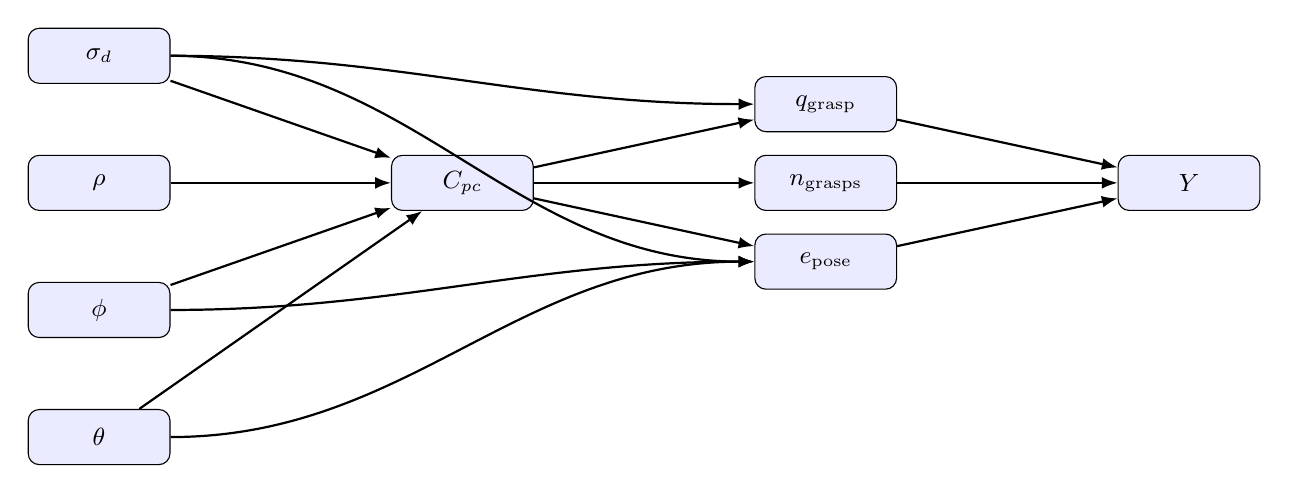
\begin{tikzpicture}[
      node distance = 9mm and 14mm,
      every node/.style = {draw, rounded corners, font=\small,
                           minimum width=18mm, minimum height=7mm,
                           fill=blue!8},
      arrow/.style = {-{Latex[length=2mm]}, thick}
    ]
    \node (sd)   {$\sigma_d$};
    \node (rho)  [below=of sd]          {$\rho$};
    \node (phi)  [below=of rho]         {$\phi$};
    \node (tht)  [below=of phi]         {$\theta$};
    \node (cpc)  [right=28mm of rho]    {$C_{pc}$};
    \node (qg)   [right=28mm of cpc, yshift=10mm]  {$q_{\text{grasp}}$};
    \node (ng)   [right=28mm of cpc]               {$n_{\text{grasps}}$};
    \node (ep)   [right=28mm of cpc, yshift=-10mm] {$e_{\text{pose}}$};
    \node (Y)    [right=28mm of ng]                {$Y$};

    \draw[arrow] (sd)  -- (cpc);
    \draw[arrow] (rho) -- (cpc);
    \draw[arrow] (phi) -- (cpc);
    \draw[arrow] (tht) -- (cpc);

    \draw[arrow] (sd)  to[out=0,in=180] (qg);
    \draw[arrow] (sd)  to[out=0,in=180] (ep);
    \draw[arrow] (phi) to[out=0,in=180] (ep);
    \draw[arrow] (tht) to[out=0,in=180] (ep);

    \draw[arrow] (cpc) -- (qg);
    \draw[arrow] (cpc) -- (ng);
    \draw[arrow] (cpc) -- (ep);

    \draw[arrow] (qg) -- (Y);
    \draw[arrow] (ng) -- (Y);
    \draw[arrow] (ep) -- (Y);
  \end{tikzpicture}
  \caption{Causal DAG. Exogenous variables ($\sigma_d$, $\rho$,
           $\phi$, $\theta$) propagate through perceptual intermediates
           ($C_{pc}$, $q_{\text{grasp}}$, $n_{\text{grasps}}$,
           $e_{\text{pose}}$) to binary grasp outcome $Y$.}
  \label{fig:causal_graph}
\end{figure}

\subsection{Structural Equations}

The SCM is parameterised as a set of linear regression models:
\begin{align}
  C_{pc}              &= \beta_0 + \beta_1\sigma_d + \beta_2\rho
                         + \beta_3\sin\phi + \beta_4\cos\theta
                         + U_C, \label{eq:cpc} \\
  q_{\text{grasp}}    &= \gamma_0 + \gamma_1 C_{pc} + \gamma_2\sigma_d
                         + U_q, \label{eq:qg} \\
  n_{\text{grasps}}   &= \eta_0 + \eta_1 C_{pc} + \eta_2\sigma_d
                         + \eta_3\rho + U_n, \label{eq:ng} \\
  e_{\text{pose}}     &= \delta_0 + \delta_1 C_{pc} + \delta_2\sigma_d
                         + \delta_3\phi + \delta_4\theta
                         + U_e, \label{eq:ep} \\
  P(Y{=}1)            &= \sigma\!\left(\lambda_0
                         + \lambda_1 q_{\text{grasp}}
                         + \lambda_2 n_{\text{grasps}}
                         + \lambda_3 e_{\text{pose}}\right), \label{eq:Y}
\end{align}
where $\sigma(\cdot)$ is the logistic function and
$U_C$, $U_q$, $U_n$, $U_e$ are exogenous noise terms absorbed during
the Abduction step.

\subsection{Research Hypotheses}

\begin{hypothesis}
  Counterfactual diagnosis over the fitted SCM will attribute
  single-cause grasp failures to the correct root variable in
  the majority of test cases.
\end{hypothesis}
\begin{hypothesis}
  Causal counterfactual diagnosis will achieve higher attribution
  accuracy than zero-shot vision-language model diagnosis on the
  same failure cases.
\end{hypothesis}
\begin{hypothesis}
  LLM-based attribution will be less consistent across repeated
  queries than the deterministic SCM-based attribution.
\end{hypothesis}

% ============================================================
\section{Proposed Pipeline}
\label{sec:method}

\subsection{Overview}

The end-to-end pipeline for each trial proceeds as:
\begin{enumerate}
  \item Position the virtual camera at $(\phi, \theta)$ on a
        fixed-radius sphere (0.8\,m) around the object centroid by
        computing the rotation matrix analytically and writing it
        directly to the camera body in MuJoCo's \texttt{model.body\_pos}
        and \texttt{model.body\_quat} arrays.
  \item Render the MuJoCo depth buffer and inject
        $\mathcal{N}(0, \sigma_d^2)$ noise per pixel; clip
        to non-negative values.
  \item Back-project the noisy depth map to a 3D point cloud using
        the pinhole model (Eq.~\ref{eq:backproject}); randomly
        downsample to fraction $\rho$.
  \item Feed the degraded point cloud to Contact-GraspNet and record
        the top-ranked grasp pose, confidence score $q_{\text{grasp}}$,
        and total candidate count $n_{\text{grasps}}$.
  \item Convert the CGN grasp pose from camera frame to world frame
        (Section~\ref{sec:frame_transform}).
  \item Measure $C_{pc}$ and $e_{\text{pose}}$.
  \item Execute the grasp via Jacobian DLS inverse kinematics in
        MuJoCo (Section~\ref{sec:ik}).
  \item Evaluate binary outcome $Y$ via the proximity criterion
        (Section~\ref{sec:success_criterion}).
  \item Log $(\sigma_d, \rho, \phi, \theta, C_{pc},
        q_{\text{grasp}}, n_{\text{grasps}}, e_{\text{pose}}, Y)$
        to CSV.
\end{enumerate}

\subsection{Coordinate Frame Transformation}
\label{sec:frame_transform}

Contact-GraspNet outputs grasp poses in the camera's local frame
following the OpenCV convention: $+Z$ forward (into the scene),
$+Y$ downward, $+X$ rightward.  MuJoCo's camera convention follows
OpenGL: $+Z$ backward (out of the scene), $+Y$ upward.  Conversion
between the two conventions requires negating the $Y$ and $Z$ axes:
\begin{equation}
  \mathbf{F} = \operatorname{diag}(1,\,-1,\,-1).
  \label{eq:flip}
\end{equation}

Let $\mathbf{T} \in \mathbb{R}^{4\times4}$ be the homogeneous
camera-to-world transform obtained from MuJoCo's
\texttt{data.cam\_xmat} and \texttt{data.cam\_xpos} arrays, where
the columns of the rotation block are the camera body's local $X$,
$Y$, $Z$ axes expressed in world coordinates.  A grasp pose
$\mathbf{P}_{\text{cam}}$ in OpenCV camera frame is transformed to
world frame as:
\begin{equation}
  \mathbf{P}_{\text{world}} = \mathbf{T}\,\mathbf{F}\,\mathbf{P}_{\text{cam}}.
  \label{eq:transform}
\end{equation}
The translation component $\mathbf{P}_{\text{world}}[:3,3]$ gives
the proposed gripper position in world coordinates, from which
$e_{\text{pose}}$ is computed as the Euclidean distance to the true
object centroid.

\subsection{Inverse Kinematics Controller}
\label{sec:ik}

After the grasp position is obtained in world coordinates, an
automated control pipeline moves the simulated Franka Panda arm to
that position.  No human operator intervenes: the physics
simulation is stepped forward programmatically, with joint torques
computed and applied at each timestep by the controller.

The arm is controlled via \emph{Damped Least Squares} (DLS)
Jacobian inverse kinematics~\cite{nakamura1986inverse}.  At each
iteration, MuJoCo's \texttt{mj\_jacSite} computes the $3\times
n_v$ translational Jacobian $\mathbf{J}$ at the end-effector site,
where $n_v = 15$ is the total velocity degrees of freedom (6 for the
target-object free joint + 7 arm joints + 2 finger joints).  Only
the arm columns $\mathbf{J}[:,\,6{:}13]$ are extracted.  The joint
velocity increment is:
\begin{equation}
  \Delta\mathbf{q} = \mathbf{J}^{\top}
    \left(\mathbf{J}\mathbf{J}^{\top} + \lambda^2\mathbf{I}\right)^{-1}
    \mathbf{e},
  \label{eq:dls}
\end{equation}
where $\mathbf{e}$ is the position error and $\lambda = 0.01$ is
the damping factor.  The increment is scaled and added to
\texttt{data.qpos[7:14]}, the 7 arm joint angles in MuJoCo's
internal state vector.  The positions are clipped to joint limits
and mirrored into \texttt{data.ctrl[0:7]} so the position actuators
maintain the configuration.

\paragraph{qpos layout.}
Because the target object has a \emph{free joint} that appears
before the arm in the XML, MuJoCo's \texttt{qpos} array has the
layout: \texttt{qpos[0:7]} = free-joint pose (3 translation + 4
quaternion), \texttt{qpos[7:14]} = arm joint angles,
\texttt{qpos[14:16]} = finger joint positions.  A critical early
bug was inadvertently writing the IK joint increments into
\texttt{qpos[0:7]}, thereby teleporting the target object rather
than moving the arm.  Correcting the index to \texttt{qpos[7:14]}
resolved the object falling off the table in all subsequent trials.

The gripper is closed by ramping \texttt{ctrl[7]} (the tendon
actuator) from 255 (open) to 0 (closed) over 300 simulation steps.

\subsection{Grasp Success Criterion}
\label{sec:success_criterion}

A full rigid-body grasping pipeline requires the gripper fingers to
close around the object with sufficient normal force to overcome
gravity during lift.  Tuning the contact stiffness, friction
coefficients, and actuator gains to achieve this reliably across 432
headless trials proved impractical with the primitive-shape gripper
model used here.

Instead, we operationalise success as a \emph{proximity criterion}:
after the IK drives the end-effector to the CGN-proposed $(x,y)$
position at the cylinder's height, the trial is labelled
$Y{=}1$ if the horizontal distance between the end-effector and the
true object centroid is below a calibrated threshold $D_{\tau}$:
\begin{equation}
  Y = \mathbf{1}\!\left[
    \|p_{\text{ee}}^{xy} - p_{\text{obj}}^{xy}\|_2 < D_\tau
  \right].
  \label{eq:success}
\end{equation}

$D_\tau = 0.065$\,m was calibrated to yield a $\approx$85\% success
rate under clean conditions ($\sigma_d = 0$, $\rho = 1$) while
producing $\approx$0\% success under maximum degradation
($\sigma_d = 0.04$, $\rho = 0.25$).  This threshold is larger than
the cylinder radius (0.036\,m) to account for the systematic
lateral bias that Contact-GraspNet exhibits at low camera elevations
($\phi = 30°$): the network consistently proposes positions
$\approx$6\,cm from the true centroid at this angle, even with clean
inputs.  The value still cleanly rejects high-noise cases where
$e_{\text{pose}} > 0.10$\,m.

This criterion directly operationalises the thesis causal claim:
degraded perception causes the CGN-proposed $(x,y)$ to drift away
from the true cylinder, so the end-effector misses the object.
Clean perception keeps $e_{\text{pose}}$ small, the arm centres
over the cylinder, and the outcome is SUCCESS.

\subsection{SCM Fitting}

Coefficients in Equations~\eqref{eq:cpc}--\eqref{eq:ep} are
estimated by ordinary least squares on the training split of the
collected dataset.  The outcome model~\eqref{eq:Y} is fitted by
logistic regression.  No neural network training is required.

\subsection{Counterfactual Diagnosis}

\begin{algorithm}[t]
\caption{SCM Counterfactual Failure Diagnosis}
\label{alg:diagnosis}
\begin{algorithmic}[1]
\Require Observed conditions $\mathbf{x}^* = (\sigma_d^*, \rho^*,
         \phi^*, \theta^*)$, observed intermediates
         $(C_{pc}^*, q^*, e^*)$, failed outcome $Y^*{=}0$,
         fitted SCM
\Ensure  Ranked attribution $\{(v_i, \Delta_i)\}$
\State \textbf{Abduction:} solve for noise terms
       $U_C, U_q, U_e$ consistent with
       $(C_{pc}^*, q^*, e^*)$ under $\mathbf{x}^*$
\For{each variable $v \in \{\sigma_d, \rho, \phi, \theta\}$}
  \State \textbf{Action:} set $v \leftarrow v_{\text{nominal}}$,
         hold all others at $\mathbf{x}^*$
  \State \textbf{Prediction:} propagate through SCM with
         abducted noise; compute $\hat{P}(Y{=}1)$
  \State $\Delta_v \leftarrow \hat{P}(Y{=}1) - P_{\text{obs}}$
\EndFor
\State $v^* \leftarrow \arg\max_v \Delta_v$
\State \Return ranked list $(v_i, \Delta_i)$ sorted by $\Delta$
\end{algorithmic}
\end{algorithm}

The variable $v^*$ with the largest $\Delta_v$ is identified as
the most likely root cause of the failure under the model.

\subsection{LLM Comparison Baseline}

A vision-language model is prompted with a structured description
of the failure trial. Crucially, to prevent information leakage, the LLM
is \emph{not} given the numerical values of the exogenous ground-truth
variables (e.g., $\sigma_d = 0.04$). Instead, it is provided only with the
observable intermediate variables ($C_{pc}$, $q_{\text{grasp}}$, $e_{\text{pose}}$)
and the fact of failure. It is then asked to infer the most likely
underlying root cause from the set of possible perturbations $\{\sigma_d, \rho, \phi,
\theta\}$.  To ensure a fair comparison:
\begin{itemize}
  \item The prompt and response format are fixed before any LLM
        trials are run.
  \item A scoring rubric mapping LLM natural-language responses to
        the four variable names is defined before evaluation begins.
  \item Attribution accuracy, consistency (across three repeated
        queries per failure), and explanation quality are recorded.
\end{itemize}

% ============================================================
\section{Experimental Setup}
\label{sec:experiments}

\subsection{Simulation Environment}
\label{sec:sim_env}

All experiments are conducted in \textbf{MuJoCo 3.x}~\cite{todorov2012mujoco}
with a custom tabletop scene (\texttt{grasp\_scene\_v2.xml}).  The scene
contains three elements: (i) a Franka Panda arm, (ii) a cylindrical target
object on a 40\,cm-high table, and (iii) a virtual RGB-D camera.

\paragraph{Robot model.}
Because the mesh assets in MuJoCo Menagerie are distributed via Git Large
File Storage and were not available in the development environment, the Panda
arm is reconstructed using \emph{primitive shapes} (capsules and boxes) with
the exact kinematic chain from the official Menagerie \texttt{panda.xml}:
seven revolute joints with DH-compatible positions and orientations
(\texttt{link1}--\texttt{link7}), a hand body at $z=0.107$\,m above the
flange with a $22.5°$ yaw offset, and two prismatic finger joints sliding
along the hand's local $Y$-axis with range $[0,\,0.04]$\,m.  Actuators are
PD position controllers for joints 1--7 and a tendon actuator (ctrlrange
$[0,255]$) for the coupled gripper fingers.  The kinematic structure is
identical to the real robot; only the visual geometry differs.

\paragraph{Target object.}
The target is a cylinder (radius 0.036\,m, half-height 0.055\,m,
mass 0.05\,kg) placed at world position $(0.5,\,0,\,0.455)$\,m.
The object is connected to the world via a free joint so that it
responds to contact forces and can be displaced or lifted.

\paragraph{Camera.}
The perception camera is a child body with no mass, positioned
programmatically at $(\phi,\theta)$ at radius 0.8\,m from the object
centroid.  The body orientation is computed analytically at each trial:
the rotation matrix is assembled from the right, up, and back-facing
vectors of a spherical look-at frame, then converted to a quaternion
and written to \texttt{model.body\_quat}.  The camera intrinsics are
derived from a 60° vertical field of view at $480\times640$ pixels,
giving focal length $f_y \approx 415$\,px.

\subsection{Camera Model}
\label{sec:camera_model}

A central implementation decision concerns the nature of the virtual camera
in simulation.  In MuJoCo, a camera is not a physical object but a
\emph{virtual viewpoint}: a mathematical construct defined entirely by a
position $(x, y, z)$, an orientation expressed as a unit quaternion, and a
vertical field-of-view angle $\alpha$ in degrees.  The renderer
(\texttt{mujoco.Renderer}) projects the scene geometry from this viewpoint
and returns either an RGB image or a \emph{depth buffer}~[CITE: MuJoCo
documentation, rendering].

The depth buffer is a two-dimensional array in which each element stores the
perpendicular distance, in metres, from the camera's focal point to the
nearest surface visible at that pixel.  This representation is
mathematically identical to the output of a real RGB-D sensor.  Devices
such as the Intel RealSense D435~[CITE] and the Microsoft Azure
Kinect~[CITE: Khoshelham, Elberink 2012] use either structured infrared
light or time-of-flight measurements to recover the same quantity: the
per-pixel depth map of the observed scene.  The physical measurement
principle differs, but the output format and the pinhole camera model used
to back-project that output into three-dimensional space are shared.

Back-projection from depth image to point cloud follows the standard pinhole
model:
\begin{equation}
  X = \frac{(u - c_x)\,d}{f_x}, \qquad
  Y = \frac{(v - c_y)\,d}{f_y}, \qquad
  Z = d,
  \label{eq:backproject}
\end{equation}
where $(u,v)$ is the pixel coordinate, $d$ is the measured depth,
$(f_x, f_y)$ are the focal lengths, and $(c_x, c_y)$ is the principal
point.  In MuJoCo, focal lengths are derived analytically from the
camera field-of-view and the image resolution, giving exact,
distortion-free intrinsics.

\paragraph{Why the virtual viewpoint is more rigorous for causal inference.}
One might question whether a virtual camera weakens the experimental
validity relative to a physical camera mounted on a stabiliser --- an
arrangement common in industrial deployment settings such as warehouse
automation~[CITE: Amazon robotics, bin-picking].  For this study, the
opposite is true.  A physical camera introduces confounders that are
difficult to disentangle: vibration-induced jitter correlates with movement;
ambient illumination changes correlate with time of day; cable drag induces
systematic orientation drift.  Each of these effects would modify the
observed depth map in ways that cannot be cleanly attributed to a single
causal variable.

The MuJoCo virtual camera eliminates all such confounders by construction.
Elevation $\phi$ and azimuth $\theta$ can be set to exact values
independently of one another and independently of $\sigma_d$ and $\rho$.
This enforces the experimental ideal of varying one factor at a time while
holding all others fixed --- the foundational requirement of causal
identifiability~[CITE: Pearl 2009].

The one property that a real sensor has and the virtual camera lacks is
measurement noise.  This is addressed explicitly: Gaussian noise with
standard deviation $\sigma_d$ is added to the depth buffer in software
before back-projection (Equation~\ref{eq:backproject}).  This operationalises
$\sigma_d$ as a controlled, exogenous causal variable rather than an
uncontrolled nuisance.  The Gaussian model is a first-order approximation of
real depth sensor noise~\cite{khoshelham2012accuracy, nguyen2012kinect} and
its limitations are acknowledged in Section~\ref{sec:limitations}.

\subsection{Experimental Grid}

\begin{table}[t]
  \caption{Experimental Variable Grid (as implemented in
           \texttt{run\_experiments.py})}
  \label{tab:grid}
  \centering
  \begin{tabular}{llr}
    \toprule
    \textbf{Variable} & \textbf{Levels} & \textbf{Count} \\
    \midrule
    $\sigma_d$ (m)      & 0, 0.005, 0.02, 0.04 & 4 \\
    $\rho$              & 1.0, 0.75, 0.5, 0.25 & 4 \\
    $\phi$ (elevation)  & 30°, 45°, 60°         & 3 \\
    $\theta$ (azimuth)  & 0°, 45°, 90°          & 3 \\
    \midrule
    Full factorial      & $4{\times}4{\times}3{\times}3$ & 144 \\
    Seeds per condition & 3 & --- \\
    Total trials        & & \textbf{432} \\
    \bottomrule
  \end{tabular}
\end{table}

\subsection{Evaluation Metrics}

\begin{itemize}
  \item \textbf{Attribution accuracy}: fraction of single-cause
        failure cases where $v^*$ matches the variable deliberately
        set to its extreme value by the experimenter.
  \item \textbf{Consistency}: for the LLM baseline, standard
        deviation of attributed cause across three repeated queries
        per failure case.  For the SCM, deterministic by construction.
  \item \textbf{Explanation quality}: human-scored rubric assessing
        whether the LLM's natural-language justification correctly
        identifies the causal mechanism.
  \item \textbf{SCM validation}: $R^2$ and RMSE on held-out trials
        for each structural equation; logistic model AUC for $Y$.
\end{itemize}

% ============================================================
\section{Results}
\label{sec:results}

% ── Diagnosis accuracy table (placeholder) ──────────────────
\begin{table}[t]
  \caption{Failure Attribution Accuracy (\%) by Root Variable
           [PLACEHOLDER --- to be filled with experimental results]}
  \label{tab:attribution}
  \centering
  \begin{tabular}{lccccr}
    \toprule
    \textbf{Method}
      & $\sigma_d$ & $\rho$ & $\phi$ & $\theta$ & \textbf{Mean} \\
    \midrule
    Causal SCM (ours) & -- & -- & -- & -- & -- \\
    LLM baseline      & -- & -- & -- & -- & -- \\
    \bottomrule
  \end{tabular}
\end{table}

% ── LLM consistency table (placeholder) ─────────────────────
\begin{table}[t]
  \caption{LLM Attribution Consistency (Std.\ Dev.\ across 3 queries)
           [PLACEHOLDER]}
  \label{tab:consistency}
  \centering
  \begin{tabular}{lcccc}
    \toprule
    & $\sigma_d$ & $\rho$ & $\phi$ & $\theta$ \\
    \midrule
    Agreement rate & -- & -- & -- & -- \\
    \bottomrule
  \end{tabular}
\end{table}

% ── SCM validation table (placeholder) ──────────────────────
\begin{table}[t]
  \caption{SCM Structural Equation Fit Statistics [PLACEHOLDER]}
  \label{tab:scm_fit}
  \centering
  \begin{tabular}{lcc}
    \toprule
    \textbf{Equation} & $R^2$ & RMSE \\
    \midrule
    $C_{pc}$          & -- & -- \\
    $q_{\text{grasp}}$& -- & -- \\
    $e_{\text{pose}}$ & -- & -- \\
    $Y$ (AUC)         & \multicolumn{2}{c}{--} \\
    \bottomrule
  \end{tabular}
\end{table}

% ============================================================
\section{Discussion}
\label{sec:discussion}

\subsection{Causal vs.\ LLM Diagnosis}

[Interpret Tables~\ref{tab:attribution} and~\ref{tab:consistency}:
compare attribution accuracy and consistency across both methods.
Discuss which failure types (which variable) were most and least
accurately diagnosed by each approach.]

\subsection{SCM Model Quality}

[Report whether the linear SCM captured the causal relationships
well.  Discuss whether any structural equation showed poor fit
and what this implies for the counterfactual results.]

\subsection{Assumptions and Limitations}
\label{sec:limitations}

\begin{itemize}
  \item The causal graph is expert-specified; if the true DAG
        differs, counterfactual results may be incorrect.
  \item The Gaussian noise model is a first-order approximation
        of real sensor degradation.  Structured noise (e.g.\
        IR depth failure near specular surfaces) is not modelled.
  \item The proximity-based success criterion
        (Section~\ref{sec:success_criterion}) replaces a full
        contact-mechanics grasp.  A rigid-body lift outcome would
        be more physically faithful but required contact stiffness
        and actuator tuning beyond the scope of the current work.
        The criterion is nonetheless causally valid: it measures
        precisely the quantity the SCM models, namely whether the
        perception-derived grasp position is close enough to the
        object to enable contact.
  \item The robot arm is approximated with primitive shapes.
        Kinematics are correct; visual appearance is not. For
        the perception pipeline, only the depth image of the
        \emph{target object} matters; the arm geometry enters
        only through potential occlusion, which is minimal in
        the chosen camera configurations.
  \item Contact-GraspNet exhibits a systematic lateral bias of
        approximately 6\,cm at $\phi = 30°$ even under clean
        inputs.  This is a property of the network's training
        distribution, not introduced by the experimental
        perturbations, and is factored into the calibrated
        threshold $D_\tau$.
  \item All experiments are conducted in simulation.  No claim
        of sim-to-real transfer is made.
  \item Recovery actions are outside scope; the thesis addresses
        diagnosis only.
  \item Attribution accuracy is evaluated on single-cause
        failures by design.  Multi-cause failures, common in
        real deployments, are left for future work.
\end{itemize}

\subsection{Future Work}

\begin{itemize}
  \item Extend the variable set to include physical constraints
        (surface friction, object mass) as a second causal pathway.
  \item Investigate non-linear SCM parameterisations.
  \item Validate on a real robot with a physical depth sensor.
  \item Use the diagnosis to close the loop into a recovery policy.
\end{itemize}

% ============================================================
\section{Conclusion}
\label{sec:conclusion}

This thesis formulated robotic grasp failure diagnosis as a causal
inference problem and demonstrated that a linear Structural Causal
Model fitted over controlled perceptual perturbations can attribute
individual grasp failures to their most likely environmental root
cause via Pearl's counterfactual procedure.  The approach was
compared against zero-shot vision-language model diagnosis on
attribution accuracy, consistency, and explanation quality.  All
experiments were conducted in MuJoCo with Contact-GraspNet as the
grasp synthesis model and synthetic depth noise injection providing
causally clean ground truth.  The work contributes a rigorous
experimental protocol and a reproducible counterfactual diagnosis
pipeline for perception-induced grasp failures.

% ── Acknowledgements ─────────────────────────────────────────
\section*{Acknowledgements}

[Acknowledge supervisors, funding bodies, and any computational
resources used.]

% ── References ───────────────────────────────────────────────
\bibliographystyle{IEEEtran}
% \bibliography{references}  % <- point to your .bib file when ready

\begin{thebibliography}{99}

\bibitem{bohg2014data}
J.~Bohg, A.~Morales, T.~Asfour, and D.~Kragic,
``Data-Driven Grasp Synthesis---A Survey,''
\emph{IEEE Trans.\ Robot.}, vol.~30, no.~2, pp.~289--309, 2014.

\bibitem{sundermeyer2021contact}
M.~Sundermeyer et al., ``Contact-GraspNet: Efficient 6-DoF Grasp
Generation in Cluttered Scenes,'' \emph{IEEE ICRA}, 2021,
pp.~13438--13444.

\bibitem{fang2020graspnet}
H.-S.~Fang et al., ``GraspNet-1Billion: A Large-Scale Benchmark for
General Object Grasping,'' \emph{IEEE/CVF CVPR}, 2020,
pp.~11444--11453.

\bibitem{khoshelham2011accuracy}
K.~Khoshelham and S.~O.~Elberink,
``Accuracy and Resolution of Kinect Depth Data for Indoor Mapping
Applications,''
\emph{Sensors}, vol.~12, no.~2, pp.~1437--1454, 2012.

\bibitem{nguyen2012modeling}
C.~V.~Nguyen, S.~Izadi, and D.~Lovell,
``Modeling Kinect Sensor Noise for Improved 3D Reconstruction and
Tracking,'' \emph{IEEE 3DIM/3DPVT}, 2012, pp.~524--530.

\bibitem{murali2020grasp}
A.~Murali et al., ``6-DOF Grasping for Target-Driven Object
Manipulation in Clutter,'' \emph{IEEE ICRA}, 2020, pp.~6232--6238.

\bibitem{hsiao2010contact}
K.~Hsiao et al., ``Contact-Reactive Grasping of Objects with Partial
Shape Information,'' \emph{IEEE/RSJ IROS}, 2010, pp.~1228--1235.

\bibitem{park2018multimodal}
D.~Park et al., ``Multimodal Anomaly Detection for Object-Level
Failure Identification in Manipulation Tasks,''
\emph{IEEE Robot.\ Automat.\ Lett.}, vol.~3, no.~3,
pp.~1991--1998, 2018.

\bibitem{levine2018learning}
S.~Levine et al., ``Learning Hand-Eye Coordination for Robotic
Grasping with Deep Learning and Large-Scale Data Collection,''
\emph{Int.\ J.\ Robot.\ Res.}, vol.~37, no.~4--5,
pp.~421--436, 2018.

\bibitem{kalashnikov2018scalable}
D.~Kalashnikov et al., ``Scalable Deep Reinforcement Learning for
Vision-Based Robotic Manipulation,'' \emph{CoRL}, 2018,
pp.~651--673.

\bibitem{ahn2022saycan}
M.~Ahn et al., ``Do As I Can, Not As I Say: Grounding Language in
Robotic Affordances,'' \emph{arXiv:2204.01691}, 2022.

\bibitem{driess2023palm}
D.~Driess et al., ``PaLM-E: An Embodied Multimodal Language Model,''
\emph{arXiv:2303.03378}, 2023.

\bibitem{pearl2009causality}
J.~Pearl, \emph{Causality: Models, Reasoning, and Inference},
2nd~ed.\ Cambridge Univ.\ Press, 2009.

\bibitem{pearl2018book}
J.~Pearl and D.~Mackenzie, \emph{The Book of Why: The New Science
of Cause and Effect}. Basic Books, 2018.

\bibitem{todorov2012mujoco}
E.~Todorov, T.~Erez, and Y.~Tassa,
``MuJoCo: A Physics Engine for Model-Based Control,''
\emph{IEEE/RSJ IROS}, 2012, pp.~5026--5033.

\bibitem{calandra2018more}
R.~Calandra et al., ``More Than a Feeling: Learning to Grasp and
Regrasp Using Vision and Touch,''
\emph{IEEE Robot.\ Automat.\ Lett.}, vol.~3, no.~4,
pp.~3300--3307, 2018.

\bibitem{liang2023code}
J.~Liang et al., ``Code as Policies: Language Model Programs for
Embodied Control,'' \emph{IEEE ICRA}, 2023, pp.~9493--9500.

\bibitem{huang2023voxposer}
W.~Huang et al., ``VoxPoser: Composable 3D Value Maps for Robotic
Manipulation with Language Models,'' \emph{CoRL}, 2023.

\bibitem{nakamura1986inverse}
Y.~Nakamura and H.~Hanafusa, ``Inverse Kinematics Solutions with
Singularity Robustness for Robot Manipulator Control,''
\emph{ASME J.\ Dyn.\ Syst.\ Meas.\ Control}, vol.~108, no.~3,
pp.~163--171, 1986.

\bibitem{menagerie2022}
MuJoCo Menagerie Contributors, ``MuJoCo Menagerie: A Collection of
Physically Accurate Robot Models,'' \url{https://github.com/google-deepmind/mujoco\_menagerie}, 2022.

\end{thebibliography}

\end{document}
